\chapter{About the cover}
\begin{wrapfigure}{r}{0.5\textwidth}
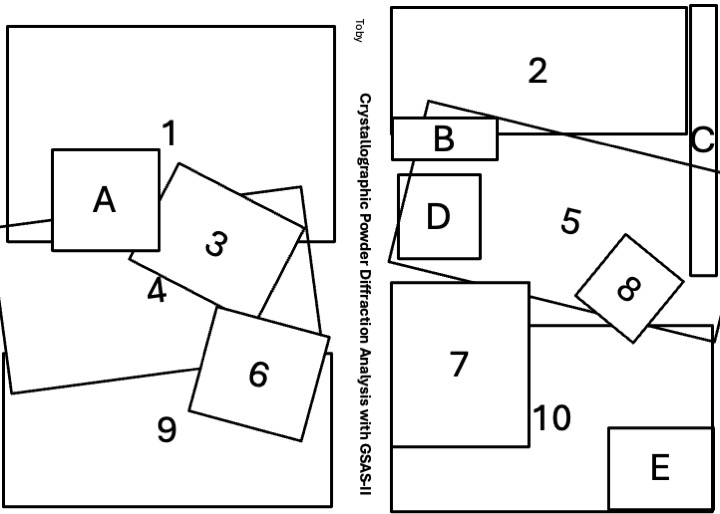
\includegraphics[width=0.9\linewidth]{figures/BookCover2.jpg}
    %\caption{Enter Caption}
    %\label{fig:placeholder}
\end{wrapfigure}

The art on the cover was all created using the GSAS-II package, and used in 2019 for the cover of \textit{Reflexions}, the American Crystallographic Association's quarterly newsletter, when Robert B. Von Dreele and Brian H. Toby were awarded the Kenneth Trueblood Award. Most were submitted by users in response to a request for interesting figures generated with GSAS-II. 

\vspace{\baselineskip}\noindent The credits for the figures are:
\begin{enumerate}
    \item 
Kent Griffith: Operando synchrotron diffraction data during electrochemical discharge and charge of high-rate lithium-ion battery electrodes comprising complex niobium tungsten oxides. Data from APS beamline 17-BM. (Griffith et al. Nature, 2018, 559, 556-563.)

    \item 
Georgiy Akopov (Kirill Kovnir Group): "Sunrise in a Forest of Peaks." Heating and cooling of a metal tetrel pnictide, synthesized during a reaction of a pre-arc-melted cerium monosilicide and phosphorus, APS 17-BM.

    \item 
Gabriela B. Gonz\'{a}lez: area detector measurements for indium oxide thin films. (Gonz\'{a}lez et al., J. Appl. Phys. 121, 205306, APS 1-ID)

    \item 
Shannon Lee (Kovnir Group): heating and cooling of a metal tetrel pnictide in a Sn flux, APS 17-BM 

    \item 
Vanessa Peterson, Christophe Didier, Zaiping Guo, \& Wei Kong Pang: Sequential neutron diffraction data from a commercial battery during cycling. WOMBAT (ACNS, Australia)

    \item 
Riley Hanus: Anisotropic strain in PbTe. This figure explained the origin of the internal-strain that softens the material’s elastic moduli. (Hanus et al. Adv. Mater. 2019, 1900108)

    \item 
Sergey Ushakov: Cubic to hexagonal phase transformation in Er\textsubscript{2}O\textsubscript{3} above 2000 °C from diffraction on a laser heated levitated sample, collected at APS 6-ID-D.

    \item 
Matt Kramer: Detail from Spinodal decomposition of Fe-Co-Al-Ni alloy, as cooled from 1250 to 800 C, APS 1-ID

    \item 
Bryan Owens-Baird (Kovnir group): variable temperature reaction of Cs\textsubscript{x}Sb\textsubscript{y}, Zn\textsubscript{8}Sb\textsubscript{7}, and Sb to form a single phase Cs\textsubscript{8}Zn\textsubscript{18}Sb\textsubscript{28} clathrate structure at circa 450 C, APS 17-BM 

    \item 
Ivan Trussov: Interesting phase transitions in sodium super-ionic conductor (NASICON)
\end{enumerate}

\noindent The other figures were generated by Bob to showcase some of the other types of graphics available in GSAS-II:

\renewcommand{\theenumi}{\Alph{enumi}}
\renewcommand{\labelenumi}{\theenumi.}
\begin{enumerate}

    \item 
An electron density contour map of Na benzoate made from structure factors extracted from powder data superimposed on its three-dimensional structure (data from Peter Stephens)

    \item 
The four-dimensional modulated structure of $\rm Na_2CO_3$. This figure is actually a movie, but I do not have the appropriate technology from Harry Potter to show that. 

    \item 
GSAS-II charge flipping result for solving structure of mcgovernite with an 8 x 8 x 200 Å rhombohedral unit cell using high resolution powder data from APS 11-BM (with Charles Lake).

    \item 
A three-dimensional structure of Mn\textsubscript{3}O\textsubscript{4} (hausmannite) with superimposed magnetic spins, solved via web interface between GSAS-II and k-SUBGROUPSMAG (Bilbao Crystallographic Server)

    \item 
A $\tau$-y slice in the xyz$\tau$ space from a four-dimensional charge-flipping structure solution map for $\rm Na_2CO_3$ showing modulation of one Na atom position.
\end{enumerate}
